\documentclass{article}

% if you need to pass options to natbib, use, e.g.:
%     \PassOptionsToPackage{numbers, compress}{natbib}
% before loading neurips_2019

% ready for submission
% \usepackage{neurips_2019}

% to compile a preprint version, e.g., for submission to arXiv, add add the
% [preprint] option:
%     \usepackage[preprint]{neurips_2019}

% to compile a camera-ready version, add the [final] option, e.g.:
\usepackage[final]{neurips_2019}

% to avoid loading the natbib package, add option nonatbib:
\usepackage[nonatbib]{neurips_2019}
\usepackage{comment}
\usepackage[utf8]{inputenc} % allow utf-8 input
\usepackage[T1]{fontenc}    % use 8-bit T1 fonts
\usepackage{hyperref}       % hyperlinks
\usepackage{url}            % simple URL typesetting
\usepackage{booktabs}       % professional-quality tables
\usepackage{amsfonts}       % blackboard math symbols
\usepackage{nicefrac}       % compact symbols for 1/2, etc.
\usepackage{microtype}      % microtypography
\usepackage{bold-extra}
\usepackage{amsmath}
\usepackage{graphicx}
\usepackage{subfig}
\usepackage{array}

\title{Overparameterization, Batch Norm, and the Attack of the Confused Gradients}

% The \author macro works with any number of authors. There are two commands
% used to separate the names and addresses of multiple authors: \And and \AND.
%
% Using \And between authors leaves it to LaTeX to determine where to break the
% lines. Using \AND forces a line break at that point. So, if LaTeX puts 3 of 4
% authors names on the first line, and the last on the second line, try using
% \AND instead of \And before the third author name.
\author{
  Zongkai Tian \\
  Department of Computer Science\\
  Columbia University\\
  116 th St & Broadway, New York, NY 10027 \\
  \texttt{zt2218@columbia.edu} \\
  % examples of more authors
  \And
   James Shin\\
   Department of Computer Science\\
   Columbia University\\
   116 th St & Broadway, New York, NY 10027 \\
  \texttt{js4785@columbia.edu} \\
  \AND
  Ruisi Wang\\
  Department of Computer Science\\
  Columbia University\\
  116 th St & Broadway, New York, NY 10027 \\
  \texttt{rw2720@columbia.edu} \\
  % \And
  % Coauthor \\
  % Affiliation \\
  % Address \\
  % \texttt{email} \\
  % \And
  % Coauthor \\
  % Affiliation \\
  % Address \\
  % \texttt{email} \\
}

\begin{document}

\maketitle
% \begin{abstract}
% \textit{Overparameterization}
% \end{abstract}

\begin{abstract}
\textit{In this paper, we aim to give a richer theoretical understanding of precisely why overparameterization and batch normalization allow for quicker convergence to global and local optima during training. Overparameterization and batch normalization has been shown extensively to work well in practice in terms of speeding up training. However, many of these empirical works that focus on building network architectures do not capture the theoretical essence behind why and how these methods work in practice. In this paper, we answer this question by diving into how each respective method works from a rich theoretical perspective. First, we present a quantity known as ``gradient confusion'' from recent research work by Sankararaman et al. \cite{gradient_confusion}, and we show how it directly correlates to training speed. Second, we show how several methods (such as overparameterization and batch normalization) share the characteristic of having low gradient confusion. Third, we dive deeper into the theoretical and experimental aspects of both overparameterization and batch normalization in order to show precisely why training speeds are enhanced via these methods, and how they work to lower gradient confusion.}
\end{abstract}

\section{Introduction}
Neural networks have seen remarkable progress in recent years in terms of approximating complex functions using various optimization methods such as stochastic gradient descent. In particular, neural networks in practice have shown how \textit{overparameterization} (an increase in parameters of a model over the number of training data) and \textit{batch normalization}, are able to make complex neural networks easier to train. However, prior to recent research, not much was understood in terms of concretely defining why these methods work so well to speed up training. \textbf{Why, precisely, do overparameterization and batch normalization allow for quicker convergence to global and local minima?} Many papers showcase these results empirically rather than from a theoretical perspective. In this paper we address this question by investigating a recently-developed concept known as \textit{gradient confusion}, a measure of differences between stochastic gradients of each data sample in a training set, that causes convergence to slow down. We also will discuss overparameterization and batch normalization in-depth, which can be shown (both empirically and theoretically) to lower gradient confusion and thus speed up training.

This paper is divided into three subparts: Gradient confusion, overparameterization, and batch normalization. We also have broken the discussion of each subpart into three sections. Firstly, we describe each respective problem setup by defining terms; secondly, we describe existing theoretical and experimental work in order to justify each concept's importance (while also describing any new theoretical expressions, findings, notes, or corrections along the way); thirdly, we describe our own findings from crafted experiments. To conclude, we discuss our own appreciations and reservations for each of the topics.


\section{Gradient Confusion}
\subsection{What is Gradient Confusion?}
We first define gradient confusion in the context of stochastic gradient descent (SGD). Given $N$ training points $X = x_1,...,x_N$, we proceed with gradient descent, back-propagating for each training point. Using these training points, we can specify $N$ loss functions, $\{f\}_{i \in [N]}$. Then we use SGD to solve the empirical risk minimization problem; that is, we hope to find optimal solution
$$w^* = \text{arg min}_{w \in \mathbb{R}^d} \frac{1}{N} \sum_{i=1}^N f_i (w).$$
Then for iteration $k$ of the algorithm, a uniformly-random example and its loss function $\nabla \tilde{f}_k$ is used to update the weights.
$$w_{k+1} = w_k - \alpha_k \nabla \tilde{f}_k(w_k)$$

As SGD stochastically chooses a training example and performs gradient updates, on iteration $k$, the selected gradient $\nabla \tilde{f}_k$ for training example $x_k$ may very well be negatively correlated with another gradient term $\nabla f_j$ for example $x_j$. This negative correlation is said to have high \textit{gradient confusion}, a quantity introduced by Sankararaman, et al. \cite{gradient_confusion}. \\

More formally, a set of objective functions $\{f_i\}_{i \in [N]}$ is said to have a $\textit{gradient confusion bound}$ $\eta \geq 0$ if, for fixed $w \in \mathbb{R}^d$,

$$ \langle \nabla f_i(w), \nabla f_j(w) \rangle \geq -\eta, \;\; \forall i \not = j \in [N]$$

That is, the inner product of the gradient vectors of every pair of unique loss functions is bounded by $-\eta$. Throughout the rest of this paper, we will use \textit{gradient confusion} to refer to the gradient inner product shown here.

Intuitively, when we have a gradient confusion bound $-\eta$ that is positive, or a very small negative value, we say that there is ``low gradient confusion.'' This case would imply that an epoch of SGD over an entire dataset leads to faster training, because most of the gradient updates of the weights would have components that are aligned with each other. On the other hand, if gradient confusion bound $-\eta$ is a large negative value, we say there is ``high gradient confusion,'' which leads to slower training.

In practice, in high dimensions, \textit{randomly-chosen vectors are nearly orthogonal with high probability} \cite{Milman}; so, we might reasonably expect the \textit{average} randomly-chosen set of training examples to have approximately orthogonal gradients, as long as the number of parameters is large, and the number of training data is small, in order to minimize the probability of encountering gradient confusion. 

This may hold on expectation, but it is difficult to ensure low gradient confusion without more rigorous reasoning. We also do not have any guarantees that these gradient vectors will behave truly randomly over the course of the SGD algorithm. As such, we present general theories and guarantees of overparameterizing and batch-normalizing a network, as well as empirical experiments, in order to show that low gradient confusion indeed holds. This analysis would then concretely explain why training is sped up when these methods are employed, and also hopefully shed light into how methods can be designed in order to speed up training, which is an incredibly expensive task.

\subsection{Existing theory: Network layer width and gradient confusion}
Consider a simple two-layer linear network $g(\textbf{x}) = \textbf{W}_1 \textbf{W}_0 \textbf{x}$, with $\textbf{x} \in \mathbb{R}^d$, $g(\textbf{x}) \in \mathbb{R}$, $\textbf{W}_1 \in \mathbb{R}^{l \times d}$, and $\textbf{W}_0 \in \mathbb{R}^{1 \times l}$. Also, suppose element $w_{ij} \stackrel{}{\sim} \text{Normal}(0, 1/l)$, $\forall w_{ij} \in \textbf{W}_0, \textbf{W}_1$, and also $x_i \in \textbf{x} \stackrel{}{\sim} \text{Normal}(0, 1/d)$. Chen, et al. \cite{chen} provides the following bounds for expected value and variance of the inner product:
$$\mathbb{E}_{\textbf{W}, \textbf{x}}[\langle \nabla f_i, \nabla f_j \rangle] = \Theta(\frac{1}{l}), \;\; \forall x_i, x_j$$
$$\text{var}_{\textbf{W}, \textbf{x}}(\langle \nabla f_i, \nabla f_j \rangle) \leq \mathbb{E}_{\mathbf{W}, \mathbf{x}} [||\nabla f_i||^2 ||\nabla f_j||]^2 = O(\frac{1}{l^2})$$

\begin{figure}[h]
	\centering
    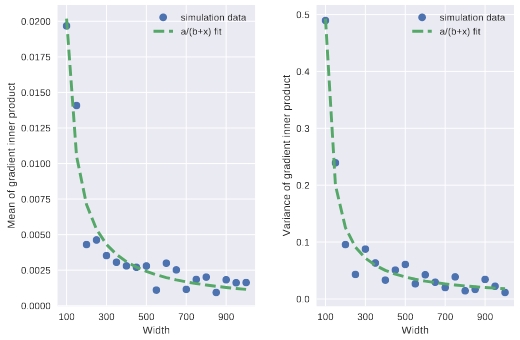
\includegraphics[width=0.5\textwidth]{pics/overparameterization/grad_inner_prod_exp_var.png}
	\caption{Simulation by Sankararaman et al. \cite{gradient_confusion} showing the mean and variance of gradient inner products for linear neural networks.}
	\label{fig:mean_inner_prod}
\end{figure}

This implies that width $l$ and gradient confusion have an inverse relationship. The proof can be found in the appendix of Chen, et al. \cite{chen}. The paper also showcases experiments of which we abbreviate here in Fig. \ref{fig:mean_inner_prod}, showcasing the relationship between network width and gradient confusion. They used a fully-connected 5-layer linear neural network of input dimension $d = 100$, where each layer took on the width specified in the graph. Both mean and variance of the gradient inner products decrease at a rate of $O(1/l)$, thus verifying the bounds above.

\subsection{A direct application of Chebyshev's inequality for a new expressive result.}
We now directly apply Chebyshev's inequality to the provided expressions for expected value and variance of the gradient inner products in order to get a \textit{new} expression that more precisely captures the implications behind these bounds:
$$\boxed{\mathbf{P}\left( \left\lvert \langle \nabla f_i, \nabla f_j \rangle - \Theta(\frac{1}{l}) \right\rvert \geq \epsilon  \right) \leq \frac{1}{\epsilon^2}O(\frac{1}{l^2}), \;\; \forall i \not = j \in [N]}$$
As width $l$ of the middle layer is increased, terms $\Theta(1/l)$ and $O(1/l^2)$ approximate to zero. This shows that the probability of the inner product of any two gradients of the losses deviating greatly from zero is very small. That is, as the width increases, the gradient inner products concentrate more towards zero, and therefore become more deterministic; this deterministic behavior of gradients with width overparameterization agrees with the findings of other works \cite{oymak}, \cite{bassily}, \cite{SimonDu}.\\

\begin{figure}[h]
	\centering
    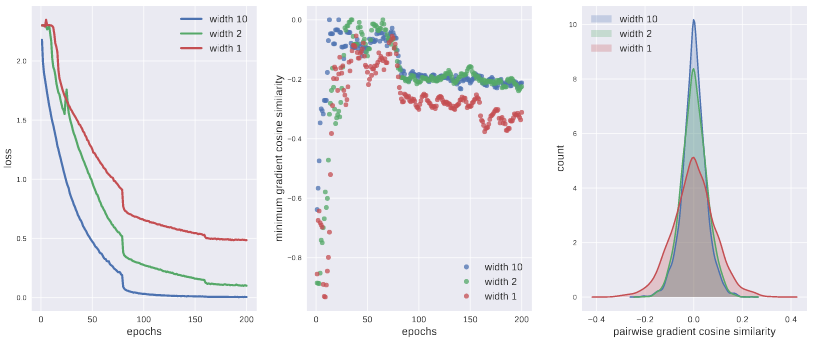
\includegraphics[width=0.75\textwidth]{pics/overparameterization/grad_consine_sim.png}
	\caption{Sankararaman et al. \cite{gradient_confusion} showcasing the effects of overparameterization on gradient confusion.}
	\label{fig:grad_cosine_sim}
\end{figure}

The experiments shown by Sankararaman et al. \cite{gradient_confusion} in Fig. \ref{fig:grad_cosine_sim} verify these results on networks with increasing widths. The left plot shows convergence speeding up with increasing width. The middle plot shows minimum gradient cosine similarities, which shows gradients becoming more and more orthogonal with increasing width, thus making training easier. The right plot shows a histogram of pairwise gradient cosine similarities; more width causes more gradients to become concentrated towards zero, as our application of Chebyshev's inequality suggests. This experiment also verifies that the results hold for multilayer linear networks; interested readers are encouraged to read about similar bounds by Chen et al. \cite{chen} for bounds on multilayer linear networks, and 2-layer non-linear networks.

As such, overparameterizing a network by increasing width certainly reduces gradient confusion, thus leading to faster training time. In order to precisely understand why this is the case from an optimization point of view, we dive deeper into work by S. Du, et al \cite{SimonDu}, which discusses how gradient descent can improve training and provably optimize overparameterized networks.

\section{Overparameterization}
\subsection{Problem description: what is overparameterization?}
We survey previous research work on optimization and generalization of two-layer neural networks, which mainly focus on how they converge to global minimum and generalize in the overparameterized setting -- a setting in which the number of parameters in a network is beyond the number of training data. To investigate convergence guarantees to global minima, and study about speed of convergence, we focus on a paper by Du \cite{SimonDu} which talks about how overparameterization causes the Gram matrix\footnote{Given a set $V$ of $m$ vectors (points in $R^n$), the Gram matrix $G$ is the matrix of all possible inner products of $V$, i.e. $G_{i j}=v_i^T v_j$.}  ($H(x)$) to remain positive-definite and hold a lower-bounded least-eigenvalue that guarantees the linear convergence to global minima. Soundry and Carmon \cite{SoudryCarmon} analyze the properties of differentiable local minima (DLMs) of the mean square error loss (MSE) for mild overparameterization and guarantees zero training loss for single-hidden-layer and multiple-hidden-layer cases. Arora \cite{Arora} refines the analysis of Du \cite{SimonDu} by introducing larger widths, and proves why true labels will converge faster than random labels. 
%Arora also discusses generalization bounds; Weinan \cite{Weinan1} \cite{Weinan2} furthers the discussion on generalization bounds as well. 

For experiments, we refer to Du \cite{SimonDu} by varying widths in order to prove that overparameterization can significantly improve the convergence rate, and make the percentile of pattern and maximum distance from initialization of weights smaller. Then, we set up our own experiments to reproduce these results, as well as experiment with much more neurons to see whether these patterns still hold from a different view. 

\subsection{Existing theoretical background}
Du \cite{SimonDu} addresses that for any non-convex and non-smooth optimization objective function, and even with random labels, randomly-initialized first-order methods such as stochastic gradient descent are still guaranteed to converge to zero training loss and find global minimums.\\

Du's theoretical work involves both continuous time analysis and discrete time analysis. We first focus on continuous time analysis to prove several key theorems. To set the foundation for discussion, first we define the concept of gradient flow, which represents gradient descent with infinitesimal steps. Formally, it is defined:
\begin{center}
    $\frac{d W_r(t)}{dt} = -\frac{\partial L(w(t),a)}{\partial W_r(t)}$
\end{center}

The main theorem for the convergence rate of gradient flow has four main assumptions, which encompass the following.
\begin{itemize}
\item No two inputs are parallel, and the Gram matrix $H(x)$ has a positive minimum eigenvalue.
\item The data is scaled; that is, $\|x_i\|_{2} = 1$, and $|y_i|\leq C$. As noted, these assumptions are only for simplification purposes, and Du uses bounded labels to match most real-world data sets.  
\item Overparameterization holds for our model: $m=\Omega(\frac{n^6}{\lambda^4_0 \sigma^3})$.
\item Random initialization is used; namely, the elements of $W$ are initialized i.i.d. as $w_r\sim N(0,I)$, and $a_r \sim \text{Uniform}[{-1,1}]$.
\end{itemize}

\textbf{Theorem.} (Du et al. \cite{SimonDu}). For $r \in [m]$, with probability at least $1-\sigma$ over this initialization,
\begin{center}
    $\|u(t)-y\|^2_2 \leq \text{exp}(-\lambda_0 t)\|u(0)-y\|^2_2$.
\end{center}

What this theorem shows is that, if $m$ is large enough, the training error $u(t)$ will guaranteed converge to 0 at an exponential rate. 

There are four main lemmas to prove this theorem. Firstly, they utilize arc-consine kernels and the law of the large numbers. 
It is not hard to show that elements of the Gram matrix $\mathbf{H(t)}=\{H_{ij}(t)\}$ satisfy the following function:
\begin{center}
    $H_{ij}(t) = \frac{1}{m} x_i^T x_j\sum_{r=1}^{m}\Pi\left\{ x_i^T w_r(t)\geq 0,x_j^T w_r(t)\geq 0\right\}$
\end{center}
If $m$ is large enough, the initial random state becomes approximately close to trained weights; that is, $W(t)\approx W$. Then, $H(t) \approx H(0) \approx H^{\infty}$. In this case, the derivative of the predicted value can then written as 
\begin{center}
    $\frac{d u(t)}{dt} = H(t)(y-u(t)) \approx H^{\infty}(y-u(t))$
\end{center}
With these foundations addressed above, Lemma 1 by Du shows that $H(0)$ and $H^{\infty}$ are close due to the Law of Large Numbers, and that the least eigenvalue of $H(0)$ is lower-bounded with high probability. Lemma 2 makes a further step and points out that if weights $w_r(t)$ are stable, $H(t)$ becomes close to $H^{\infty}$ as well. Lemma 3 shows that, if the eigenvalue of $H(t)$ is lower-bounded, the loss converges at a exponential convergence rate, and the weights at $t$ become close to initialized weights. Lemma 4 expands Lemma 3 to a wider realm of $\mathbb{R}$ to fit in all $t$. \\ 

Similar to continuous time analysis, discrete time analysis also comes to the conclusion that, with probability at least $1-\sigma$ over the initialization, we have 
\begin{center}
    $\|u(t)-y\|^2_2 \leq (1-\frac{\eta \lambda_0}{2})^k\|u(0)-y\|^2_2$
\end{center}

Arora \cite{Arora} refines the analysis of Du \cite{SimonDu} by showing that with overparameterized nets, it becomes trivial to achieve a training error of zero, even without properly labeled data. \\

\textbf{Theorem.} Suppose $\kappa$ is the magnitude of the training loss in each iteration. Assume $\lambda_0 = \lambda_{min} H^{\infty} > 0, \kappa = O (\frac{\epsilon\sigma}{\sqrt{n}})$,$m = \Omega(\frac{n^7}{\lambda_0^4 \kappa^2\sigma^4\epsilon^2})$, and $\eta = O(\frac{\lambda_0}{n^2})$. Then with probability at least $1-\sigma$ over the random initialization, for all $k = 0,1,2 …$,
\begin{center}
    $\|y-u(k)\|_2 = \sqrt{\sum_{i=1}^n (1-\eta\lambda_i)^{2k} (V_i^T y)^2}\pm\epsilon$
\end{center}

The theorem above shows how fast $(1-\eta\lambda_i)^{2k} (V_i^T y)^2$ converges to 0 as $k$ grows. When $k = 0$, it starts at $(V_i^T y)^2$. Then, it decreases at a rate of $(1-\eta\lambda_i)^{2k}$. The larger $(1-\eta\lambda_i)^{2k} (V_i^T y)^2$ is, the faster $\lambda_i$ decreases to 0. In this case, as label $y$ can be decomposed into its projection to $H^{\infty}$ 's eigenvectors, we have that $\|y\|_2^2 = \sum_{i=1}^n{(V_i^T y)^2}$. And, as mentioned above, in order to achieve faster convergence, the projection of $u$ onto the top eigenvectors is expected to be larger. Based on this rule, for a set of labels $y$, if the amount that the true labels align with the top eigenvectors $(V_i^T y)^2$ is large, then gradient descent will converge quickly. With random labels, the projections of eigenvectors are uniform,  thus gradient descent converges rather slowly. \\

\indent Different from Arora et al. \cite{Arora} and Du et al. \cite{SimonDu}, Soudry and Carmon \cite{SoudryCarmon} discuss the relationship between local and global minima. By analyzing the properties of differentiable local minima (DLMs) under mean squared error loss (MSE) and mild overparameterization, they show a guarantee of zero training loss for the single-hidden-layer and multiple-hidden-layer cases. They prove convergence to global minima for both single-hidden-layer networks and multiple-hidden-layer networks. They define mean square error (MSE) as the following:

\begin{center}
    $\frac{1}{2}\hat{E}e^2 = \frac{1}{2}\hat{E}(y-W_2 \text{diag}(a_1)W_1x)^2 = \frac{1}{2}\hat{E}(y-a_1^T \text{diag}(w_2)W_1x)^2$
\end{center}

For a single hidden layer, assume that $d$ is the width of the activation layer. Let $N$ represent the sample size let $\epsilon$ represent Gaussian dropout noise, and let $X$ be smoothed by some small Gaussian noise. Then, the theorem can be addressed as: \\\\
``\textit{If $N< d_1 d_0$, then all differentiable local minima are global minima with $\text{MSE} = 0$, and $(X,\epsilon)$ almost everywhere.} ''

Also, a similar result can be shown for any multiple-layer neural network with arbitrary depth. For any randomly-set weights of the first $L-2$ layers, every differentiable local minima (with respect to the weights of the last two layers) is also a global minimum with loss zero. 


\subsection{Existing Experiments in Other Work}

In Du's work \cite{SimonDu}, they perform experiments using synthetic data by uniformly-generating $n = 1000$ data points from a $d = 1000$-dimensional unit sphere, as well as labels from a one-dimensional standard Gaussian distribution. 
They ran 100 epochs of gradient descent with different widths $m$. \\

% \pagebreak
Figure \ref{fig:conver} shows how different $m$ affects the convergence rates; as $m$ becomes lager, convergence rate improves.

\begin{figure}[htb]
	\centering
    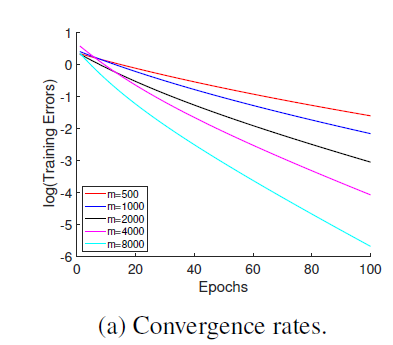
\includegraphics[scale= 0.5]{pics/overparameterization/ConvergeRate.PNG}
    \caption{Convergence Rates}
	\label{fig:conver}
\end{figure}

Figure \ref{fig:patternsample} tests the relation between different m and the number of pattern changes.

\begin{figure}[htb]
	\centering
    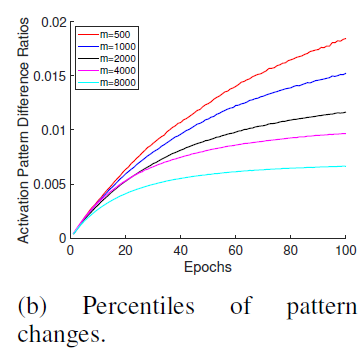
\includegraphics[scale= 0.5]{pics/overparameterization/PatternSample.PNG}
    \caption{Percentiles of pattern changes}
	\label{fig:patternsample}
\end{figure}

Figure \ref{fig:maxdistance} tests the relation between different m and maximum distances between wights vectors and their initialization.
\begin{figure}[htb]
	\centering
    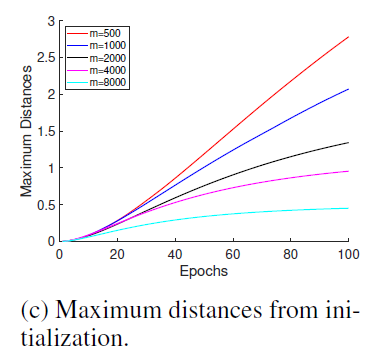
\includegraphics[scale= 0.5]{pics/overparameterization/maximumdistance.PNG}
    \caption{Maximum distances from initialization}
	\label{fig:maxdistance}
\end{figure}

So, it is generally the case that when $m$ becomes larger in an overparameterized network, convergence rates improve, thus agreeing with experiments from the gradient confusion paper by Sankararaman et al. \cite{gradient_confusion}. The percentiles of pattern changes, as well as maximum distances from initialization, also become smaller.
\\

\subsection{Our Own Experiments and Observations}

We performed our own experiments referring to Du's result \cite{SimonDu}. Our experiment generates synthetic data, with $X$ being $n = 10$ randomly-generated data points of a $d = 1000$-dimensional unit sphere. It runs with $m = 100000$ neurons, and $y$ labels from a one-dimensional standard Gaussian distribution.

In Figure \ref{fig:zeroloss}, we show that when $m$ is large enough, the training loss will converge to 0, even with completely random labels. 

\begin{figure}[htb]
	\centering
    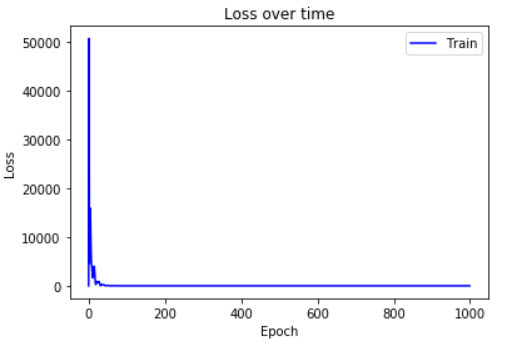
\includegraphics[scale = 0.5]{pics/overparameterization/loss_over_time_0-1k.jpg}
    \caption{Loss over time by 1-1000 epochs}
	\label{fig:zeroloss}
\end{figure}

In addition to the results shown by Figure \ref{fig:zeroloss}, Figure \ref{fig:twohundredloss} shows that when the network is overparameterized, the convergence rate is generally fast, and not many training epochs are needed, which also agrees with what we found in Sankararaman et al.'s work \cite{gradient_confusion}; gradient confusion drops with more parameters, thus speeding up training.

\begin{figure}[htb]
	\centering
    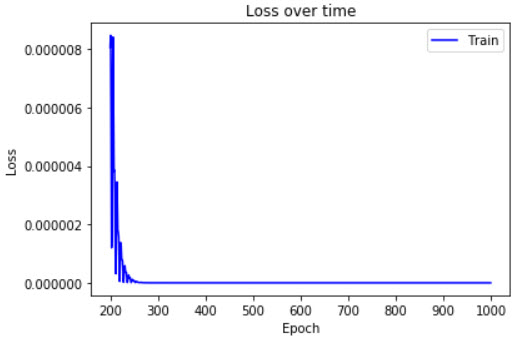
\includegraphics[scale = 0.5]{pics/overparameterization/loss_over_time_200-1k.jpg}
    \caption{Loss over time by 200-1000 epochs}
	\label{fig:twohundredloss}
\end{figure}

Lastly, Figure \ref{fig:maxdistanceloss} showcases the change of the max distance between the updated weights and its initialized values when using large $m$; the distance converges over all the epochs and converges pretty fast, which is what we expected after studying gradient confusion results. 

\begin{figure}[htb]
	\centering
    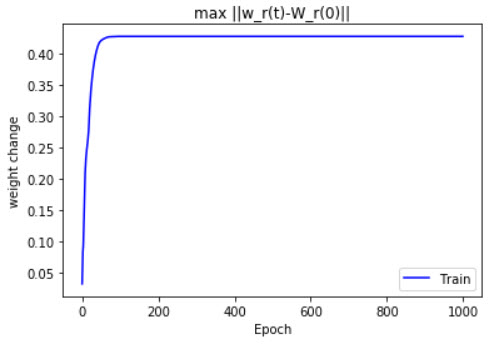
\includegraphics[scale = 0.5]{pics/overparameterization/max_weight_change.jpg}
    \caption{Maximum distances from initialization}
	\label{fig:maxdistanceloss}
\end{figure}

After studying the theory of overparameterizing as well as conducting experiments, it is now clear why convergence is achieved quickly in training, and how the results align with the results from gradient confusion; the theoretical understanding of overparameterization that we had sought in the beginning of this paper has been achieved!  In the next section, we explore a process known as batch normalization, which is a technique that is well-known for speeding up training.

\pagebreak
%This paper accurately estimate the magnitude of training loss in each iteration. The key finding is that the number of iterations needed to achieve a target accuracy depends on the projections of data labels on the eigenvectors of a certain Gram matrix. Also, it give a generalization bound for the solution found by GD, based on accurate estimates of how much the network parameters can move during optimization. The generalization bound depends on a data-dependent complexity measure and notably, is completely independent of the number of hidden units in the network.

%As to Generalization bounds, the well known VC-dimension of neural networks is at least linear in the number of parameters and therefore classical VC theory cannot explain the generalization ability of modern neural networks with more parameters than training samples. PAC-Bayes approach to compute non-vacuous generalization bounds for MNIST and ImageNet, respectively. All these bounds depend on certain properties of the trained neural networks. In the paper, one of main results shows :

%For any 1-Lipschitz loss function, the generalization error of the two-layer ReLU network found by GD is at most 
%\begin{center}
%  $\sqrt{\frac{2y^T(H^\infty)^-1y}{n}}$
%\end{center}
%In that case, fix an error parameter $\epsilon > 0$ and failure probability $\sigma \in (0,1)$ Suppose we have data $S={(x_i,y_i)}_{i=1}^n$ are i.i.d. samples from $a (\lambda_0,\frac{\sigma}{3},n)$ - non-degenerate distribution D, and $k = O(\frac{\epsilon\lambda_0\sigma}{\sqrt{n}}$,$m \geq K^{-2}poly(n,\lambda_0^{-1},\sigma^{-1},\epsilon^{-1})$.Consider any loss function $l:R*R ->[0,1]$ that is 1-Lipschitz in the first argument such that $l(y,y)=0 $Then with probability at least $1-\sigma$ over the random initialization and training examples, the two-layer neural network $f_{w(k),a}$ trained by GD for $k\geq\omega(\frac{1}{\mu^{\lambda_0}}\log{\frac{1}{\sigma_\epsilon}})$ iterations has population loss $L_D(f_{W(k),a})= E_{(x,y)~D}[l(f_{W(k)},a(X),y)]$ bounded as
%\begin{center}
%    $L_D(f{W(k),a})\leq \sqrt{\frac{2y^T(H^\infty)^-1y}{n}} +3\sqrt{\frac{\log(\frac{6}{\sigma}}){2n}}+\epsilon$
%\end{center}
%\subsection{A Priori Estimates For Two-layers Neural Networks}
%We provide a perspective for understanding why two-layer neural networks perform better than kernel methods. We focus on two -layer networks, and we consider models with explicit regularization. We establish estimates for the population risk which are symptotically sharp with constants depending only on the properties of the target function. 
%\begin{itemize}
%\item We establish a priori estimates of the population risk for learning two -layer neural networks with an explicit regulation.
%\item We make a detailed comparison between the neural network and kernel methods using these a priori estimates. 
%\end{itemize}
%For a two-layer neural network $f(x;\theta)$ of width m, we define the regularized risk as 
%\begin{center}
%  ${\MakeUppercase{J}_\lambda}(\theta) : = \hat{\MakeUppercase{L}_n}(\theta)+ \lambda(\|\theta\|_P+1)$
%\end{center}
%The +1 term at the right hand side is included only to simplify the proof. Our result also holds if we do not include this term in  the regularized risk. The corresponding regularized estimator is defined as 
%\begin{center}
%  $\hat{\theta_{n,\lambda}} = argmin{{\MakeUppercase{J}_\lambda}(\theta)}$
%\end{center}
%For any $f \in barron space(\omega)$,there exists a two-layer neural network $f(x;\hat{\theta}$ of width m with $\|\Hat{\theta}_P\leq 2\gamma_2(f)$, such that
%\begin{center}
%  $E_x[(f(x)-f(x;\Hat{\theta}))^2]\leq\frac{3\gamma_2^2(f)}{m}$
%\end{center}
%The basic intuition is that the integral representation of f allows us to approximate f by the Monte-Carlo method:$f(x) \approx\frac{1}{m}\sum_{k=1}^{m} a(w_k){\sigma(<w_k,x>)}$ where${W_k}_{k=1}^m$ are sampled from the distribution $\pi$
% main result shows 
%\begin{itemize}
%\item For noiseless case, Assume that the target function $f^* /in B_2(\omega)$ and $\lambda \geq \lambda_n$. Then for any $\sigma > 0 $ and, the probability at least $1-\sigma$ over the choice of the training set $S$, we have
%    \begin{center}
%      $E_x[(f(x;\Hat{\theta})-f^*(x))^2]\leq\frac{\gamma_2^2(f^*)}{m} +\lambda \Hat{\gamma_2}(f^*)+\frac{1}{\sqrt{n}}(\Hat{\gamma_2}(f^*)+\sqrt{\ln{\frac{n}{\sigma}}})$
%    \end{center}
%And the population risk for the kernel methods should be much larger than the population risk for the neural network.
%\item For noisy case, Assume that the target function $f^* /in B_2(\omega)$ and $\lambda \geq \lambda_n$. Then for any $\sigma > 0 $ and, the probability at least $1-\sigma$ over the choice of the training set $S$, we have
%     $E_x[(f(x;\Hat{\theta})-f^*(x))^2]\leq\frac{\gamma_2^2(f^*)}{m} +\lambda B_n \Hat{\gamma_2}(f^*)+\frac{B^2_n}{\sqrt{n}}(\Hat{\gamma_2}(f^*)+\sqrt{\ln{\frac{n}{\sigma}}})+\frac{B^2_n}{\sqrt{n}}(c_0 \sigma^2+\sqrt{\frac{E[\xi^2]}{n^{1/2}\lambda}})$
%\item For classification problem, under the same assumption as above, and taking $\lambda = \Lambda_n$, for any $\sigma \in (0,1)$, with probability at least $1-\sigma$, we have
%   \begin{center}
%     $\epsilon(\Hat{\eta}) \leq \epsilon(\eta ^*) + \frac{\gamma_2^2(f^*)}{\sqrt{m}}+\Hat{\gamma^{1/2}}(f^*)\frac{\ln^{1/4}{d}+\ln^{1/4}{\frac{n}{\sigma}})}{n^{1/4}}$
 %   \end{center}
%\end{itemize}

%And for numerical experiments, it has been tested from three aspects:
%\begin{itemize}
%\item Shape bounds for the generalization gap.

%The test accuracy of the regularized and unregularized solution are generally comparable, but the values of $\frac{\|\theta\|_P}{\sqrt{n}}$ are different. Especially, the values of the unregularized models are always several orders of magnitude larger than that for the regularized models.

%Also, by comparing of the path norms between the regularized and un-regularized solutions for varying widths, it shows for the un-regularized model this quantity increases with network width, whereas for the regularized model it is almost constant. 
%\item Dependence on the Initialization.
%By testing on $m=10000,n= 100$ and vary the variance of the random initialization $K$, it shows regularized models are much more stable than the un-regularized models. 
%\end{itemize}

%\subsection{A Comparative Analysis of the Optimization and Generalization Property of Two-layer Neural Network and Random Feature Models Under Gradient Descent Dynamics}

%Firstly, it prove that the results of Simon Du still hold, the gradient descent dynamics still converges to a global minimum exponentially fast, regardless of the quality of the labels. And functions obtained are uniformly close to the ones found in an associated kernel method, with the kernel defined by the initialization. Secondly, it prove that for target functions in the appropriate reproducing kernel Hilbert space (RKHS), the generalization error can be made small if certain early stopping strategy is adopted for the gradient descent algorithm. The conclusion can be explicit regularization is necessary for two-layer neural network models to fully realize their potential in expressing complex functional relationships. 

%The problem has been set up with the regression problem with a training data. By fitting into a two -layer neural network, the ultimate goal is to minimize the population risk and in practice, it can only work with the following empirical risk. 

%To analyse the over-parameterized case, the paper has demonstrated in four aspects:
%\begin{itemize}
%\item properties of the initialization 
%For any fixed $\sigma > 0$,with probability at least $1-\sigma$ over the random initialization, we have
 %   \begin{center}
%      $\Hat{R_n}(\theta_0)\leq {1\2}(1+c(\sigma)\sqrt{m}\beta)^2$
%    \end{center}
%where $c(\sigma) = 2+\sqrt{\ln{\frac{1}{\sigma}}}$.

%\item Gradient descent near the initialization 
%For any fixed $\sigma \in (0,1)$, assume that $m \geq \frac{8}{\lambda_n^2}\ln(\frac{2n^2}{\sigma})$.Then with probability at least $1-\sigma$ over the random choices of $\theta_0$, we have the following holds for any $t\in[0,t_0]$,
%    \begin{center}
%      $\Hat{R_n}(\theta_t)\leq e^{-m(\lambda_n^{(a)}+\beta^2\lambda_n^{(b)})}t\Hat{R_n}(\theta_0)$
%    \end{center}
    
%\item Characterization of the whole GD trajectory
%\item Curse of dimensionalality pf the implicit regularization
%\end{itemize}

%The numerical results to illustrate our theoretical analysis with two tests: 
%\begin{itemize}
%\item The first experiment studies the convergence of GD dynamics for over-parameterized two-layer neural networks with different initialization. GD algorithm for the neural network models converges exponentially fast for all initialization considered.
%\item The second experiment compares the GD dynamics of two -layer neural networks and random feature models. When the width is very small, the GD algorithm for the random feature model does not converge, while it does converge for the neural network model and the resulting model does generalize. For the intermediate width, the GD algorithm for both models converges, and it converges faster for the neural network model than for the random feature model. The test accuracy is slightly better for the resulting neural network model. When width is large, the behavior of the GD algorithm for two models is almost the same. 
%\end{itemize}

%This paper has shown that for over-parametrized two-layer neural networks without explicit regularization, the gradient descent algorithm is sufficient for the purpose of optimization. But to obtain dimension-independent error rates for generalization, one has to require that the target function be in the RKHS with a kernel defined by the initialization. Given a target function in the Barron space, in order for implicit regularization to work, one has to know before hand that kernel function for that target function and use that kernel function to initialize the GD algorithm. This requirement is certainly impractical. In the absence of suck a knowledge, one should expect to encounter the curse of dimensionality for general target function in Barron space, as is proved in this paper. 
\pagebreak
\section{BatchNorm}
\label{label:BatchNorm}

\subsection{Preliminaries and motivation}
For some motivation into why we should study batch normalization in the first place, we first reference experiments by Sankararaman et al. \cite{gradient_confusion} which show how batch normalization actually lowers gradient confusion, just like overparameterization, thus accelerating training dramatically.

\begin{figure}[h]
	\centering
    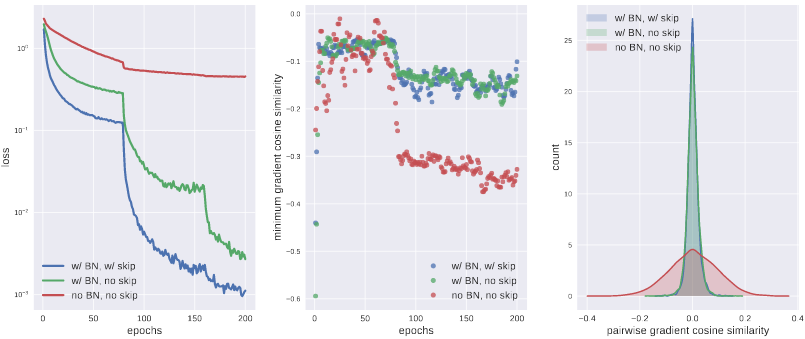
\includegraphics[width=\textwidth]{pics/batchNorm/batchnorm_grad_conf.png}
	\caption{Experiments by Sankararaman et al. \cite{gradient_confusion}. }
	\label{fig:batchnorm}
\end{figure}

Here we see experiments that showcase the effects of batch normalization on gradient confusion, similar to those shown in Figure \ref{fig:grad_cosine_sim}; in fact, the results look very similar! Note that in these graphs, Sankararaman et al. also shows results for skip connections, which should be ignored, as they are out of the scope of this paper. In the left graph, the red plot shows how a non-batch-normalized network is much less efficient in terms of loss reduction over epochs in comparison to the green plot, which is of a batch-normalized network. The middle plot shows how the minimum gradient cosine similarities become more orthogonal with the introduction of batch normalization, thus causing training to become easier over epochs. In the rightmost graph, a histogram of pairwise gradient cosine similarities is shown, with a histogram of the non-batch-normalized network shown in red, and the batch-normalized network shown in green. We also notice from the rightmost graph that the batch-normalized network has very tightly-concentrated pairwise gradient cosine similarities, implying that the gradients of the network behave similarly to random vectors that are drawn from the unit sphere, causing optimization to become much more stable in the process.

Now that we have experimentally convinced ourselves that batch normalization reduces gradient confusion and therefore enhances the efficiency of training, let us dive into the theory to gain a deeper understanding of what precisely causes this gradient confusion reduction.

\subsection{Existing theory on Batch Normalization}
\subsubsection{The Architecture of Batch Normalization}

Ioffe \& Szegedy \cite{batchnorm} originally proposed adding batch normalization (BatchNorm) as part of their network architecture. The new BatchNorm network achieved the same accuracy as a state-of-the-art image classification model, while also training 14 times faster -- this is a remarkable improvement.

BatchNorm is an algorithm that is applied to each neuron individually, within a layer of interest. Figure \ref{fig:batchnorm} shows how it works on a fully-connected network, which we explain in details below.


\begin{figure}[h]
	\centering
    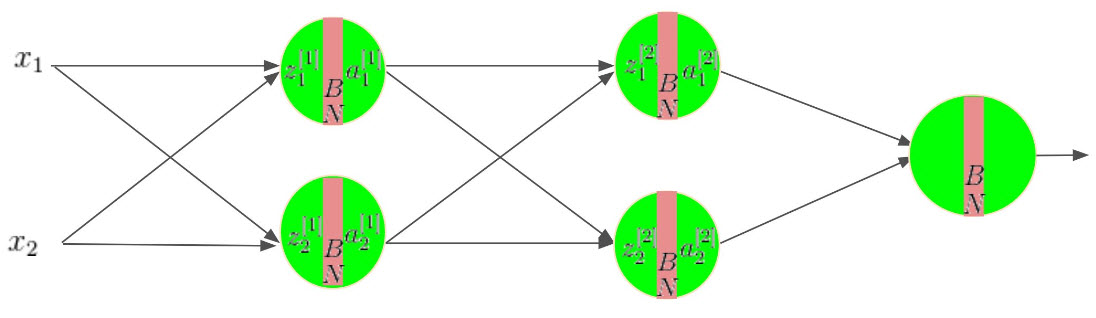
\includegraphics[width=\textwidth]{pics/batchNorm/batch-normalization.jpg}
	\caption{Batch Normalization Architecture\\Source: https://www.learnopencv.com/batch-normalization-in-deep-networks/}
	\label{fig:batchnorm}
\end{figure}

\subsubsection{Training with Batch Normalization}
In an unnormalized network, for neuron $i$ at an arbitrary layer, we have that $z_i=w_ix$, and $a_i=g(z_i)$, where $x\in\mathbb{R}^{d\times m}$ is a size $m$ mini-batch of $d$-dimensional inputs into the next layer (thus, these inputs could either be input training data, or output from previous layer), and $g$ is a non-linear activation function. So, $z_i$ is vector of size $m$. In our discussion, the bias term $b$ and the layer indices are omitted for simplicity. BatchNorm is added to each neuron as the brown slice shown in Figure \ref{fig:batchnorm} before the non-linear activation. On each individual neuron, we then calculate:
\begin{align*}
    z_i^{norm}& = \frac{z_i-\mu}{\sqrt{\sigma^2+\epsilon}}  &(1)\\
    \hat{z}_i&= \gamma_i\cdot z_i^{norm}+\beta_i  &(2)\\
    a_i&=g(\hat{z}_i) &(3)
\end{align*}

where $\mu$ and $\sigma^2$ in equation (1) above are the mean and variance of mini-batch $z_i$, respectively. They then scale and shift the normalized value $z_i^{norm}$ to ensure that not all transformed data fall under the linear regime of non-linear activation, as shown in equation (2). Here, $\gamma_i$ and $\beta_i$ are introduced as learnable parameters for each neuron.  $\epsilon$ is added for numerical stability of the calculation, i.e. to avoid errors if $\sigma \approx 0$ (the typical value for $\epsilon$ is $10^{-8}$). Note that at each step of mini-batch training, the mean and variance of $z_i$ need to be recalculated.

\subsubsection{Gradient Descent with Batch Normalization}

During the training phase, the chain rule is still applicable to a BatchNorm network. See here: for an arbitrary loss function $l$, the chain rule would be as follows:

\begin{align*}
   \frac{\partial l}{\partial z_i^{norm}} &= \frac{\partial l}{\partial \hat{z}_i}\cdot\gamma_i\\
   \frac{\partial l}{\partial \sigma^2}  &= \sum_{i=1}^m\frac{\partial l}{\partial z_i^{norm}}\cdot(z_i-\mu)\cdot\frac{-1}{2}(\sigma^2+\epsilon)^{-3/2} \\
   \frac{\partial l}{\partial \mu}  &= \sum_{i=1}^m\frac{\partial l}{\partial z_i^{norm}}\cdot \frac{-1}{\sqrt{\sigma^2+\epsilon}}\\
   \frac{\partial l}{\partial z_i}  &=  \frac{\partial l}{\partial z_i^{norm}} \cdot\bigg(\sqrt{\sigma^2+\epsilon}\bigg)^{-1} + \frac{\partial l}{\partial \sigma^2}\cdot\frac{2(z_i-\mu)}{m} +  \frac{\partial l}{\partial \mu}\cdot\frac{1}{m}\\
   \frac{\partial l}{\partial \gamma_i}  &=  \sum_{i=1}^m\frac{\partial l}{\partial \hat{z}_i}\cdot z_i^{norm} \\
   \frac{\partial l}{\partial \beta_i}  &= \sum_{i=1}^m\frac{\partial l}{\partial \hat{z}_i} \\
\end{align*}

Therefore, we can still use backpropagation to update all the parameters in a BatchNorm neural network.

\subsubsection{Inference with Batch Normalization}

Suppose the whole training data is split into $B$ mini-batches. When inference is to be performed with a BatchNorm network, a deterministic mean and variance, $\mu$ and $\sigma^2$ in Eq. (1) (independent of the mini-batch) are desired. To achieve a fixed mean and variance, once training is completed, with frozen parameters, the $B$ training mini-batches are re-processed through the trained network. Then for neuron $i$, the mean for mini-batch $k\in\{1,2,\cdots,B\}$ is denoted as $\mu_k$ and the variance as $\sigma^2_k$. Then, let
\begin{align*}
   M &= \frac{1}{B}\sum_{k=1}^B\mu_k\\
   V &= \frac{m}{m-1}\Bigg(\frac{1}{B}\sum_{k=1}^B\sigma^2_k\Bigg)\\
\end{align*}
where $M$ is the average of the means of the mini-batches, and $V$ is an unbiased estimate of the average variance of the mini-batches. Therefore, when doing inference on test data, Eq. (1) is rewritten as:

\begin{align*}
    z_i^{norm}& = \frac{z_i-M}{\sqrt{V+\epsilon}}
\end{align*}


\subsubsection{Loss-Landscape Smoothing} \label{landsmooth}
Santurkar et al. \cite{landscape} shows that the loss function landscape is smoother in BatchNorm networks. BatchNorm reduces the effective Lipschitzness constant and improves smoothness of the gradient. We discuss this in detail below.

\textbf{\subsubsubsection{Observations}}

In Santurkar et al.'s work \cite{landscape}, they perform experiments with two deep architectures: a VGG-type convolutional network with 11-19 layers (the exact number of layers is not specified in the paper) on the CIFAR10 dataset, and a 25-layer deep linear network (DLN) on synthetic Gaussian data. They also explicitly add time-varying noise of non-zero mean and non-unit-variance to each of the batch-normalized nodes independently (referred to as a "noisy" BatchNorm model in the paper) so that the distributions of activations on each node in a mini-batch is ensured to be unstable. From the performance of the VGG-type network, shown in Figure \ref{fig:vgg}, they observe that BatchNorm and noisy BatchNorm have comparable performance, and both converge faster than the standard ``vanilla'' network. However, Figure \ref{fig:vgg} shows that, although the ``noisy'' BatchNorm achieved faster training speed than the standard ``vanilla'' network, as well as comparable performance to that of BatchNorm, the weight distribution of the ``noisy'' BatchNorm  is noisier than the standard network, indicating a large ICS as defined in Ioffe \& Szegedy, 2015 \cite{batchnorm}. Also, notice that in Layer \#13, the weight distribution of BatchNorm has more ICS than the standard network.

\begin{figure}[h] 
	\centering
    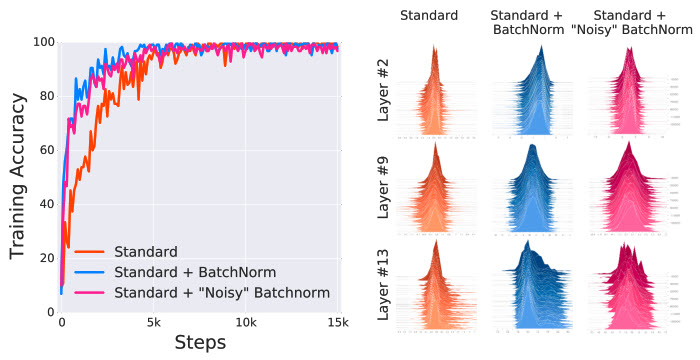
\includegraphics[scale=0.6]{pics/batchNorm/Santurkar_fig2.jpg}
	\caption{VGG Performance}
	\label{fig:vgg}
\end{figure}

The above findings seem to contradict Ioffe \& Szegedy's work \cite{batchnorm} where they claim that BatchNorm helps stabilize internal weight distributions so as to reduce ICS. To investigate why BatchNorm improves the training process, they analyze the optimization landscape in VGG-type networks and show it in Figure \ref{fig:optimizationlandscape}.

\textbf{\subsubsubsection{Experimental and Theoretical Results}}

At each training step, suppose the weights are at position $A$ of the optimization landscape. They calculate the gradient at position $A$, then ``walk'' in the gradient direction of $A$ and mark several positions along the way. In graph (a), of Figure \ref{fig:optimizationlandscape}, the shaded area is the change in loss between $A$ and each of the marked positions. In graph (b), the shaded area is the $l_2$-difference of the gradient at $A$ and the gradient at each of the marked positions. Graph (c) shows the maximum value of gradient difference (as the $l_2$-norm) divided by the distance from $A$ to the corresponding marked position. The maximum value can be seen as the ``effective'' Lipschitz constant. Through this graph, it is rather evident that BatchNorm improves smoothness of the optimization landscape.

\begin{figure}[h]
	\centering
    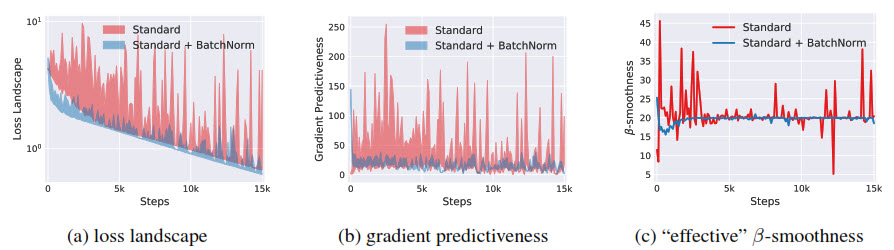
\includegraphics[width=\textwidth]{pics/batchNorm/Santurkar_fig4.jpg}
	\caption{Optimization Landscape}
	\label{fig:optimizationlandscape}
\end{figure}

In the following section, the phenomenon is explored theoretically. In the theoretical setup, a single BatchNorm layer is arbitrarily inserted at a fully-connected layer. Layer weights are denoted as $W_{ij}$. An arbitrary unnormalized loss function at the current layer is denoted as $\mathcal{L}$, and the normalized loss is denoted $\hat{\mathcal{L}}$ (and they may have downstream non-linear layers). For some input $x$, let $y=Wx$. Then, we let $\hat{y}=\text{BN}(y)$, which is the batch-normalized $y$ with mean 0 and variance 1. Then, $z=\gamma\hat{y}+\beta$ where $\gamma$ and $\beta$ are assumed to be constant for the following analysis. 

\textbf{Theorem 4.1} shows that BatchNorm improve Lipschitzness of the loss with respect to $y_j$.
\begin{align*}
	||\nabla_{y_j}\hat{\mathcal{L}}||^2&\leq\frac{\gamma^2}{\sigma^2_j}\bigg(||\nabla_{y_j}\mathcal{L}||^2
	- \frac{1}{m} \langle \mathbf{1},\nabla_{y_j}\mathcal{L} \rangle^2 
	- \frac{1}{m}\langle \nabla_{y_j}\mathcal{L}, \hat{y}_j \rangle^2 \bigg)
\end{align*}

where $\sigma_j^2$ is the variance of a batch of outputs $y_j\in\mathrm{R}^m$, and $j$ denotes an arbitrary node in the normalized layer. 

We gain intuition by reasoning about each term separately. Note that $||\nabla_{y_j} \mathcal{L}||$ here denotes the Lipschitzness of the loss. The value of $\sigma_j^2$ tends to be large in practice. The inequality utilizes an assumption that $\partial \hat{\mathcal{L}}/\partial z_j = \partial \mathcal{L}/\partial y_j$. The second term, $ \langle \mathbf{1},\nabla_{y_j}\mathcal{L} \rangle^2=\big( \sum_{k=1}^{m}\partial \mathcal{L}/\partial y_j^{(k)} \big)$, is non-negative and most likely greater than zero. The third term indicates the correlation of variable $\hat{y}_j$ and $\nabla_{y_j}\mathcal{L}$. Since they both correlate to $y_j$, this term is also greater than zero. Therefore, we can confidently say that the Lipschitzness of the loss with respect to $y_j$ is improved by BatchNorm.

Next, in \textbf{Theorem 4.4}, they transfer the above theorem to one that relates to layer weights, by using chain the rule $\frac{\partial\hat{L}}{\partial W_{.j}}=\textbf{X}^T\big(\frac{\partial\hat{L}}{\partial y_{j}}\big)$. Let $g_j=\underset{||X||\leq\lambda}{\mathrm{max}}\big|\big|\nabla_{W_{\cdot j}}\mathcal{L}\big|\big|^2$, $\hat{g}_j=\underset{||X||\leq\lambda}{\mathrm{max}}\big|\big|\nabla_{W_{\cdot j}}\hat{\mathcal{L}}\big|\big|^2$ and $\mu_{g_j}=\frac{1}{m}\langle\mathbf{1},\partial\mathcal{L}/\partial y_j\rangle$. Then,
\begin{align*}
	\hat{g}_j &\leq 
	\frac{\gamma^2}{\sigma_j^2}\Bigg(
	g_j^2 - m\lambda^2\mu^2_{g_j}-\frac{\lambda^2}{m}\langle\nabla_{y_j}\mathcal{L},\hat{y}_j\rangle^2
	\Bigg)\\
\end{align*}

(Note that in original paper, $\lambda^2$ is missing in the second term and $1/m$ is missing in the third term. We believe that this may be a mistake.)

The above theorem shows that the worst-case bound of the loss gradient with respect to layer weights also improves by applying BatchNorm.

\subsubsection{Batch Normalization: Length-direction decoupling}

Kohler et al.'s paper \cite{decoupling} shows that BatchNorm is equivalent to rewriting weights in a way that decouples its length and direction. Therefore, these two parameters of the weights can actually be trained separately.

Suppose for a binary classification problem, the training data input is $\textbf{x}\in\mathbb{R}^d$, and the label is $y\in{\pm1}$. Let $\textbf{z}=-y\textbf{x}$, let $\textbf{u}:=\mathbb{E}[\textbf{z}]$, let $\textbf{S}:=\mathbb{E}[\textbf{xx}^T]$, let $\textbf{w}$ be a weight vector on an arbitrary unit on input \textbf{x}, and let $\varphi: \mathbb{R}\xrightarrow{}\mathbb{R}$ be a non-linear function. Then the output $f(\textbf{w})$ of a unit on an input \textbf{x} is:
\begin{align*}
	f(\textbf{w})=\mathbb{E}_{\textbf{x}}\big[\varphi\big(\textbf{x}^T\textbf{w}\big)\big]
\end{align*}
When we apply BatchNorm to the unit before activation, the output becomes:
\begin{align*}
	f_{BN}(\textbf{w},\gamma,g)&=\mathbb{E}_{\textbf{x}}\big[\varphi\big(BN\big(\textbf{x}^T\textbf{w}\big)\big)\big]\\
	BN\big(\textbf{x}^T\textbf{w}\big)&=g\frac{\textbf{x}^T\textbf{w}-\mathbb{E}_{\textbf{x}}[\textbf{x}^T\textbf{w}]}{\text{var}_\textbf{x}[\textbf{x}^T\textbf{w}]^{1/2}}+\gamma
\end{align*}
Assume $\textbf{x}$ has zero mean and omit $\gamma$:
\begin{align*}
	f_{BN}(\textbf{w},g)&=\mathbb{E}_{\textbf{x}}\Big[\varphi\Big(g\frac{\textbf{x}^T\textbf{w}}{(\textbf{w}^T\textbf{Sw})^{1/2}}\Big)\Big]
\end{align*}
Now, let $||\textbf{w}||_{\textbf{S}}=(\textbf{w}^T\textbf{Sw})^{1/2}$ and define $\Tilde{\textbf{w}}:=g\frac{\textbf{w}}{||\textbf{w}||_{\textbf{S}}}$. Then we can write  $f_{BN}(\textbf{w},g)$ as:
\begin{align*}
    f_{BN}(\textbf{w},g)&=\mathbb{E}_{\textbf{x}}\Big[\varphi\big(\textbf{x}^T\Tilde{\textbf{w}}\big)\Big]
\end{align*}
Therefore, BatchNorm can be seen as reparameterizing the weight space!

\textbf{\subsubsubsection{Theoretical Results}}

In this paper they make four assumptions for further theoretical analysis:

\textbf{Assumption 1}: $\mathbb{E}_{\textbf{x}}[\textbf{x}]=0$; minimum and maximum eigenvalues of $\textbf{S}$ are $\mu>0$ and $L<\infty$, respectively. Therefore, $\textbf{S}$ is a positive-definite covariance matrix of $\textbf{x}$.

\textbf{Assumption 2}: $\textbf{z}=-y\textbf{x}$ is a multivariate Gaussian random variable with mean $\textbf{u}$ and variance $\textbf{S}-\textbf{uu}^T$.

\textbf{Assumption 3}: loss function $\varphi:\mathbb{R}\rightarrow{}\mathbb{R}$ is infinitely differentiable with a bounded derivative.

\textbf{Assumption 4}: output function $f:\mathbb{R}^d\rightarrow{}\mathbb{R}$ is $\zeta$-smooth if it is differentiable on $\mathbb{R}$ and its gradient is $\zeta$-Lipschitz. Also, they assume that $\alpha_*:=\mathrm{argmin}_{\alpha}||\nabla f(\alpha\textbf{w})||^2$ exists and is finite for all $\textbf{w}$.

The architecture setup they use for theoretical analysis is a one-hidden-layer network of $m$ neurons. The network has a loss function $l:\mathbb{R}\rightarrow{}\mathbb{R}^+$ and $F(\textbf{x},\Tilde{\textbf{W}}):=\sum_{i=1}^m\theta_i\varphi(\textbf{x}^T\Tilde{\textbf{w}}^{(i)})$ with all $\theta_i$ frozen. The goal here is:
\begin{align*}
\underset{\Tilde{\textbf{W}}}{\min}\Bigg(f_{NN}(\Tilde{\textbf{W}}):=\mathbb{E}_{y,\textbf{x}}\Big[l\Big(-yF(\textbf{x},\Tilde{\textbf{W}})\Big)\Big]\Bigg)
\end{align*}
In the paper, an odd function, $\text{tanh}(x)$, is used as activation function. Therefore, the above equation can be rewritten as:
\begin{align*}
\underset{\Tilde{\textbf{W}}}{\min}\Bigg(f_{NN}(\Tilde{\textbf{W}})=\mathbb{E}_{\textbf{z}}\Big[l\Big(F(\textbf{z},\Tilde{\textbf{W}})\Big)\Big]\Bigg)
\end{align*}
They first show in \textbf{Lemma 2} that if Assumptions 1 \& 2 are true, then a critical point (local/global minimum) $\hat{\textbf{w}}^{(i)}$ for a hidden unit $i$ satisfies the following, $\forall i=1,\cdots,m$ and scalar $\hat{c}^{(i)}$:
\begin{align*}
\hat{\textbf{w}}^{(i)}=\hat{c}^{(i)}\textbf{S}^{-1}\textbf{u}
\end{align*}
The above lemma implies that, given Gaussian inputs, the critical points of all hidden neurons are along the same direction in $\mathbb{R}^d$ space. The scalar $\hat{c}^{(i)}$ depends on $\alpha, \beta$ and $\gamma$ given later. Furthermore, the direction of a critical point is only dependent on the input into the layer. 
\begin{figure}[h]
\begin{tabular}{cc}
  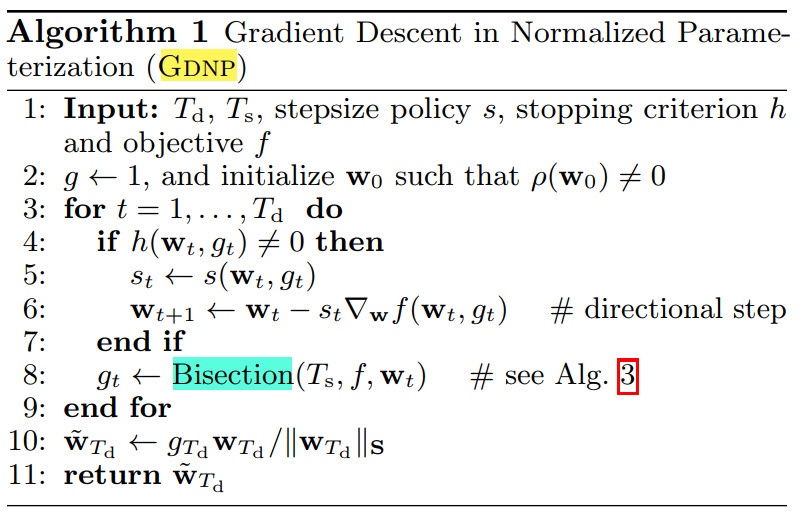
\includegraphics[scale=0.38]{pics/batchNorm/decoupling_alg1.jpg} & 
  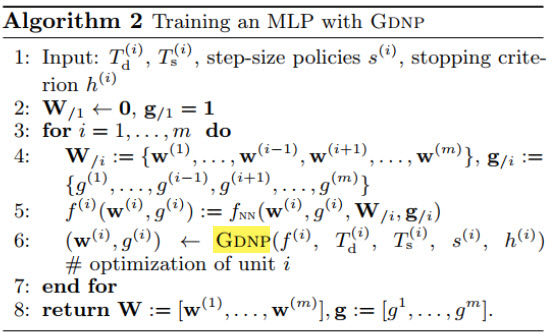
\includegraphics[scale=0.58]{pics/batchNorm/decoupling_alg2.jpg}
  \\
(1) GDNP Algorithm & (2) Training MLP with GNDP\\[6pt]
\multicolumn{2}{c}{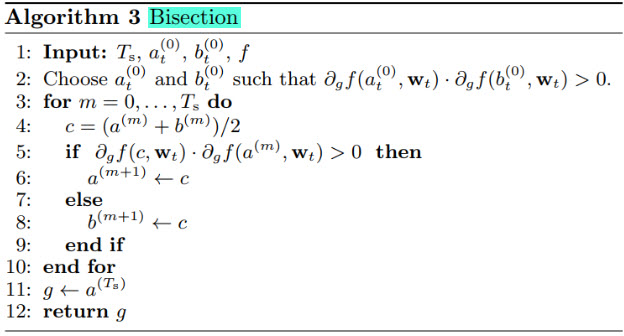
\includegraphics[scale=0.6]{pics/batchNorm/decoupling_alg3.jpg} }\\
\multicolumn{2}{c}{(3) Bisection Algorithm }
\end{tabular}
\caption{Training Algorithm}
\label{fig:algorithms}
\end{figure}
Next, they propose a training algorithm for analysis purposes, shown in Figure \ref{fig:algorithms}. The algorithm optimizes each neuron independently and sequentially (in an order of given neuron indexes). The algorithm also leverages the above \textbf{Lemma 2}, decoupling input and output of a unit. Then they prove that, if all four assumptions hold, by training with the proposed algorithm (GDNP), an exponential convergence rate can be achieved.
\begin{align*}
    ||\nabla_{\Tilde{\textbf{w}}^{(i)}}f\big(\Tilde{\textbf{w}}_t^{(i)}\big)||^2_{\textbf{S}^{-1}}&\leq(1-\mu/L)^{2t}C(\rho(\textbf{w}_0)-\rho(\textbf{w}^*))+2^{-T_s^{(i)}}\zeta|b_t^{(0)}-a_t^{(0)}|/\mu^2\\\\
    \mathrm{, where\ }\Tilde{\textbf{w}}:&=g\frac{\textbf{w}}{||\textbf{w}||_{\textbf{S}}} \mathrm{\ and\ step\ size\ } s_t^{(i)}=||\textbf{w}_i^{(i)}||^3_{\textbf{S}}/(L\theta^{(i)}g_t^{(i)}\xi_t\textbf{u}^T\textbf{w}_t^{(i)})\\
    \zeta\mathrm{\ is\ }&\mathrm{Lipschitz\ constant\ of\ }f\\\\
    C&=2\Phi^2+2i\sum_{j<i}(\theta^{(j)}c_j)^2>0\\
    \rho(\textbf{w}):&=-\frac{\textbf{w}^T\textbf{uu}^T\textbf{w}}{\textbf{w}^T\textbf{Sw}}\\\\
\end{align*}
\begin{align*}
    \xi_t&=\alpha_t^{(i)}+\sum_{j,i}\gamma_t^{(i,j)}c_j\\
    \alpha^{(i)}:&=\mathbb{E}_{\textbf{z}}\Big[l^{(1)}(F(\textbf{z},\Tilde{\textbf{W}}))\varphi^{(1)}(\textbf{z}^T\Tilde{\textbf{w}}^{(i)})\Big]-\sum_{j=1}^m\gamma^{(i,j)}(\textbf{u}^T\Tilde{\textbf{w}}^{(j)})\\
    \beta^{(i)}:&=\mathbb{E}_{\textbf{z}}\Big[l^{(1)}(F(\textbf{z},\Tilde{\textbf{W}}))\varphi^{(2)}(\textbf{z}^T\Tilde{\textbf{w}}^{(i)})\Big]\\
    \gamma^{(i,j)}:&=\theta^{(j)}\mathbb{E}_{\textbf{z}}\big[l^{(2)}(F(\textbf{z},\Tilde{\textbf{W}}))\varphi^{(1)}(\textbf{z}^T\Tilde{\textbf{w}}^{(i)})\varphi^{(1)}(\textbf{z}^T\Tilde{\textbf{w}}^{(j)})\big]\\
    \Tilde{\textbf{W}}:&=\{\Tilde{\textbf{w}}^{(1)},\cdots,\Tilde{\textbf{w}}^{(m)}\}
\end{align*}

When updating the current weight parameters $(\textbf{w}^{(i)}, g^{(i)})$, they further assume that all updated neurons weights, $\{\textbf{w}^{(k)}\}_{k<i}$, are at critical points, and that the neurons to be updated all have weight $\textbf{w}^{(k)}=\textbf{0}$ for $k>i$.

The above convergence result is actually a composition of two parts in below: convergence of the scalar $g$, and the direction $\textbf{w}$. Note that both of the two parts have exponential convergence rate.

\textbf{Convergence of scalar} $g^{(i)}$:
\begin{align*}
    \Big(\partial_{g^{(i)}}f(\textbf{w}_t^{(i)},g^{(i)}_{T_s})\Big)^2\leq2^{-T_s^{(i)}}\zeta|b_t^{(0)}-a_t^{(0)}|/\mu^2
\end{align*}
\textbf{Convergence of the direction} $\textbf{w}^{(i)}$:
\begin{align*}
    ||\textbf{w}_t^{(i)}||^2_{\textbf{S}}||\nabla_{\textbf{w}^{(i)}}f(\textbf{w}_t^{(i)},g_t^{(i)})||^2_{\textbf{S}^{-1}}\leq (1-\mu/L)^{2t}\xi_t^{2}g_t^{2}(\rho(\textbf{w}_0)-\rho(\textbf{w}^*))\\
\end{align*}

\textbf{\subsubsubsection{Experiments}}

In the experimental section, they train a neural network of 6 hidden layers with 50 neurons, each on CIFAR-10 image classification data. Note that the input data are no longer multivariate-Gaussian variables. All hidden layers are batch-normalized. For comparison, they also train an un-normalized network of the same structure. Both networks are trained by standard gradient descent and use $\text{tanh}(x)$ as middle-layer activations. To validate \textbf{Lemma 2}, i.e. the direction of the critical points is independent of downstream layers, they calculate the Frobenius norm of $\frac{\partial^2f_{NN}}{\partial\textbf{W}_4\partial\textbf{W}_i}$ as a measurement of cross-dependency of layer-4 with the other layer, layer-$i$. Their experimental results are shown in Figure \ref{fig:decouplingexperiment}. The top two graphs clearly show that BatchNorm networks achieve faster convergence rates, agreeing with what was shown in the gradient confusion experiments for BatchNorm. Also, the bottom two graphs shows that in BatchNorm networks, dependence of a middle layer on its downstream layers (layer-5 and layer-6) grows weaker as the layer becomes further away from it.

\begin{figure}[h]
	\centering
    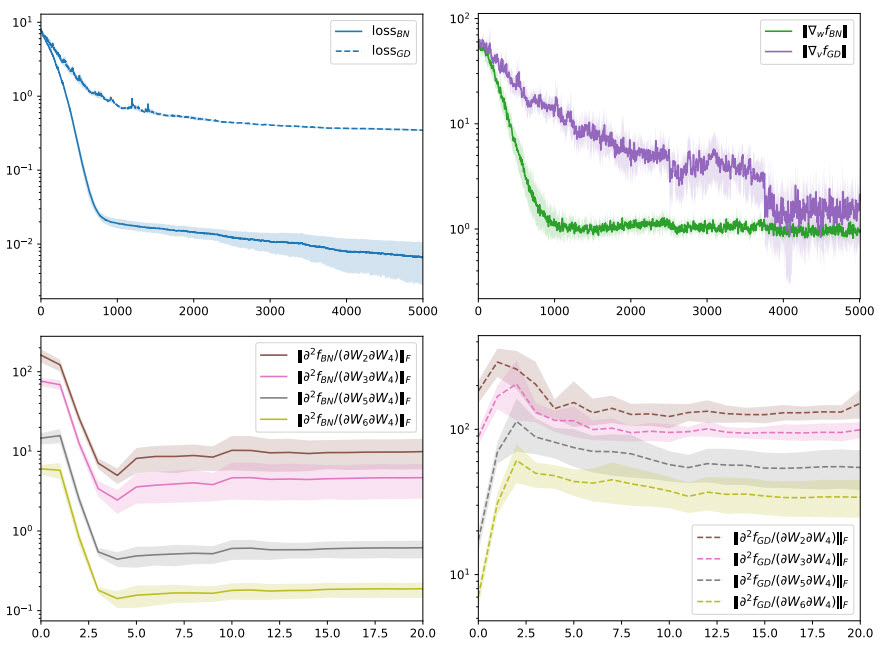
\includegraphics[scale=0.5]{pics/batchNorm/decoupling_experiment.jpg}
	\caption{Experimental Results: Top two plots show the results of the decay of the loss function as well as the norm of the loss gradient. Bottom two plots show cross-dependency in BatchNorm networks and un-normalized networks, respectively.}
	\label{fig:decouplingexperiment}
\end{figure}

\subsubsection{Variants to Batch Normalization}

\textbf{\subsubsubsection{Limitations of Batch Normalization}}

Although BatchNorm is a powerful technique that speeds up the training process, it still has its own limitations. The mean and variance of each neuron in BatchNorm depends on the size of each mini-batch, and thus varies from mini-batch to mini-batch. That would introduce certain amounts of errors that propagate through the network which is harmful to noise-sensitive applications like reinforcement learning \cite{reparameter}. Also, variance of the estimated population mean and variance is increased when the mini-batch size is small. Therefore, when applying BatchNorm, the choice of the mini-batch size should be considered carefully. Moreover, BatchNorm is not suitable for recurrent models like RNNs, which thus limits the applications of such powerful technique.

\textbf{\subsubsubsection{Weight Normalization}}

Salimans et al. \cite{reparameter} proposes Weight Normalization (WeightNorm), another way to perform neural network parameterization. In their paper, the weight vector is expressed as:
\begin{align*}
    \textbf{w}=\frac{g}{||\textbf{v}||}\textbf{v}
\end{align*}
where $g$ is a scalar, $\textbf{v}$ is a vector, and $||\textbf{v}||$ is the $L_2$ norm of $\textbf{v}$. The gradient of the loss function $l$ for a WeightNorm network, with respect to the new parameters $g$ and $\textbf{v}$, is:
\begin{align*}
    \nabla_gl &= \frac{\nabla_{\textbf{w}}l\cdot\textbf{v}}{||\textbf{v}||}\\
    \nabla_{\textbf{v}}l &= \frac{g}{||\textbf{v}||}\nabla_{\textbf{w}}l-\frac{g\nabla_gl}{||\textbf{v}||^2}\textbf{v}
\end{align*}
They also propose a ``Mean-only'' Batch Normalization method, which they adopt into the WeightNorm method. In this scheme, the pre-activation $t=\textbf{W}\cdot\textbf{x}$ is subtracted from its mean (without being scaled by its standard deviation), then applied to a non-linear activation $y=\phi(t-\mu[t])$. The parameter $\textbf{w}$ is written as a WeightNorm expression. To give some intuition into what is happening, the ``Mean-only'' BatchNorm has an effect of centering the gradient, which is a low-cost operation. In their experiments, the ``Mean-only'' WeightNorm method achieves the lowest test error among WeightNorm, BatchNorm, and regular parameterization on a CNN network. They also apply regular WeightNorm to deep convolutional variantional auto-encoders (CVAEs), a recurrent variational autoencoder with generative model (DRAW), and a Deep Q-Network (DQN) for reinforcement learning. In all three models, WeightNorm outperforms normal parameterization in terms of both convergence rate and standard evaluation metrics.

\textbf{\subsubsubsection{Layer Normalization}}

Although vanilla BatchNorm does not apply to recurrent models, not all hope is lost for more complex recurrent structures. Ba et al. \cite{layernorm} proposed a reformulation for RNNs called Layer Normalization (LayerNorm) which can be applied to networks with recurrent structures. Figure \ref{fig:batchvslayernorm} shows a comparison of BatchNorm and LayerNorm.  In an arbitrary layer, LayerNorm is applied to each input independently. 

\begin{figure}[h]
	\centering
    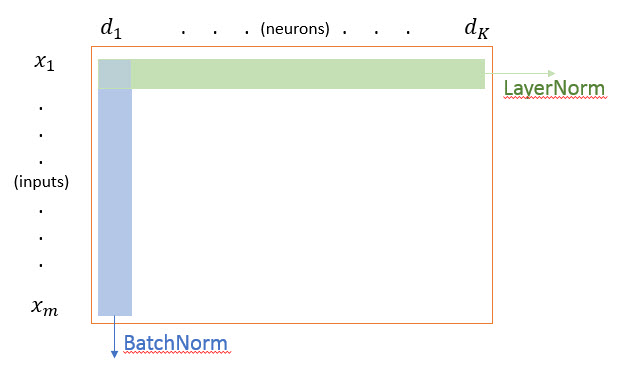
\includegraphics[scale=0.5]{pics/batchNorm/BatchNorm_vs_LayerNorm.jpg}
	\caption{Batch Normalization vs. Layer Normalization}
	\label{fig:batchvslayernorm}
\end{figure}

In a standard RNN, at timestep $t$, with current input $\textbf{x}^t$ and previous hidden state output $\textbf{h}^{t-1}$, let $\textbf{a}^t \in \mathbb{R}^K = W_{hh}\textbf{h}^{t-1}+W_{xh}\textbf{x}^t$. Then, the output $\textbf{h}^t$ can be expressed as:

\begin{align*}
    \textbf{h}^t&=\sigma\Big(\frac{\textbf{g}}{\sigma^t}\odot(\textbf{a}^t - \mu^t) + \textbf{b}\Big)\\
    \mu^t&=\frac{1}{K}\sum_{i=1}^Ka_i^t\\
    \sigma^t&=\sqrt{\frac{1}{K}\sum_{i=1}^K(a_i^t-\mu^t)^2}
\end{align*}

This model incorporates a similar idea to BatchNorm, but its expression expands to recurrent network updates. They tested this layer normalization on five tasks involving RNNs. Experimentally, all five tasks converged faster than baseline models with at least comparable results (LayerNorm perform better on three of the five tasks).

\textbf{\subsubsubsection{Group Normalization}}

Small mini-batch sizes rapidly increase BatchNorm's errors due to inaccurate estimations of population estimation statistics caused by smaller sample sizes. Thus, applying BatchNorm in large memory-consuming models that require smaller mini-batches (such as those present in computer vision tasks) is very limited, especially for image detection, segmentation, and video classification. 

Wu et al. \cite{groupnorm} tackled this weakness with the introduction of Group Normalization (GroupNorm), which is a method completely independent of mini-batch size. Implementation of GroupNorm is shown in Figure \ref{fig:groupnorm}. Calculation of the mean and variance is done on each individual input across the entire height and width of a subset of channels in a layer. The formulation is the same form as BatchNorm, the difference being which terms the sum is being done over.

\begin{figure}[h]
	\centering
    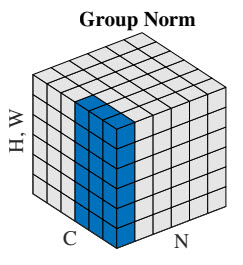
\includegraphics[scale=0.7]{pics/batchNorm/GroupNorm.jpg}
	\caption{Group Normalization: $N$ - Mini-batch size; $C$ - number of channels; $H$, $W$ - height \& width of a feature map being flattened. Normalization is taken over the blue region.}
	\label{fig:groupnorm}
\end{figure}

Figure \ref{fig:resnet} showcases how BatchNorm's performance is dependent on mini-batch size, while GroupNorm is not. The performance of GroupNorm is comparable to that of BatchNorm with larger mini-batch sizes. As for the number of channels per group, they show that in ResNet-50, all values from 2 to 64 have high performance. The value can also vary from layer to layer, which is another desirable flexibility of GroupNorm.

\begin{figure}[h]
	\centering
    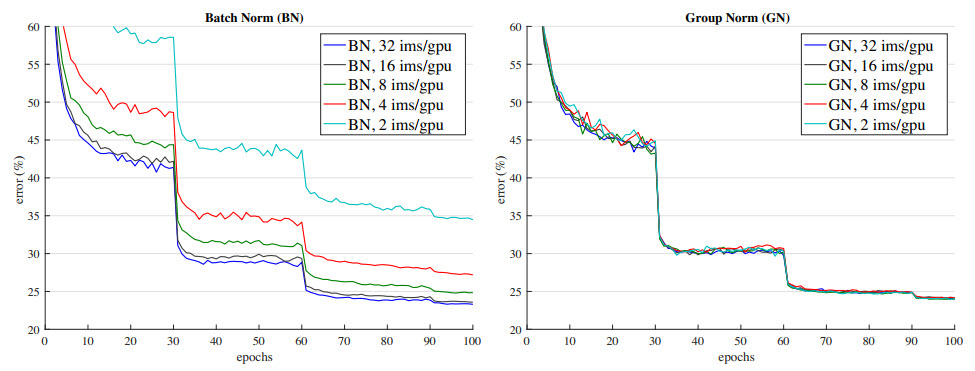
\includegraphics[scale=0.57]{pics/batchNorm/GroupNorm_vs_BatchNorm.jpg}
	\caption{ResNet-50 trained on ImageNet set}
	\label{fig:resnet}
\end{figure}

\textbf{\subsubsubsection{Summary}}

Table~\ref{normsum} shows a summary of all the mentioned normalization methods, along with their applications and calculation schemes.\\

\begingroup
\setlength{\tabcolsep}{10pt} % Default value: 6pt
\renewcommand{\arraystretch}{1.5} % Default value: 1
\begin{table}[h] 
\centering
 \begin{tabular}{|m{10em} | m{10em} | m{10em}|} 
 \hline
 Method & Application & Calculation\\  
 \hline
 Batch Normalization & Fully Connected Layers & Individual Neuron, over mini-batch input\\ [0.5ex] 
 \hline
 Layer Normalization & Recurrent Layers & Individual Input, over all neurons in a layer\\ [0.5ex]
 \hline
 Group Normalization & Convolution Layers & Individual Input, over entire height \& weight in a group of channels\\[0.5ex]
 \hline
 Weight Normalization & Any Architecture & Decouples length and direction of weights\\
 \hline
\end{tabular}
\caption{Summary of Normalization}
\label{normsum}
\end{table}
\endgroup

\subsection{Our Own Experiments}
The experiment we conducted was performed on a 7-layer fully-connected feed-forward network with 32-64-32 neurons in each hidden layer. The output layer was a softmax layer of 10 neurons, for classification. The dataset we used was Fashion-MNIST by Xiao et al. \cite{fmnist}, which is comprised of $28\times28$ pixel gray-scale images of 10 clothing categories. BatchNorm was added to all seven hidden layers. Lastly, the mini-batch size was set to 32.

Note that we added BatchNorm to all fully-connected layers. In contrast to Section \ref{landsmooth} using only a single BatchNorm layer, we sought to verify whether Lipschitzness of the loss landscape is improved when applying BatchNorm in a more practical way. We plotted the maximum loss gradient norm among batches with respect to one node in one of the middle layers, and we showcase our results in Figure \ref{fig:maxgradient}. The RELU and $\text{tanh}(x)$ activation functions were used in our experiment. The learning rate was set to 0.001 and 0.005 for each choice of activation. When the learning rate was set to 0.001, BatchNorm networks achieved comparable test accuracy as regular networks, just above 80\%. With learning rate was set to 0.005 with RELU activation, the test accuracy in the BatchNorm network was 1\% higher than the regular network (85.23\% vs. 84.26\%). Regular network using $\text{tanh}(x)$ activation failed to train at all with a learning rate of 0.005.

Given these test results, we note that when the learning rate is small (0.001), the gradient norm of the two networks has a similar landscape. However, when taking a larger learning rate (0.005), the gradient norm in BatchNorm network is smaller than that of regular networks. Also, the change of the gradient norm in BatchNorm network with training epochs is much smoother.


\begin{figure}[h]
\begin{tabular}{cc}
  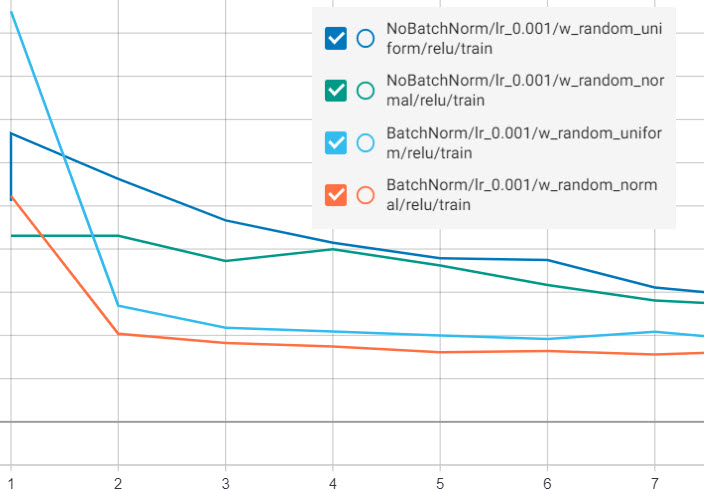
\includegraphics[scale=0.28]{pics/batchNorm/BatchNorm_relu_1.jpg} &
  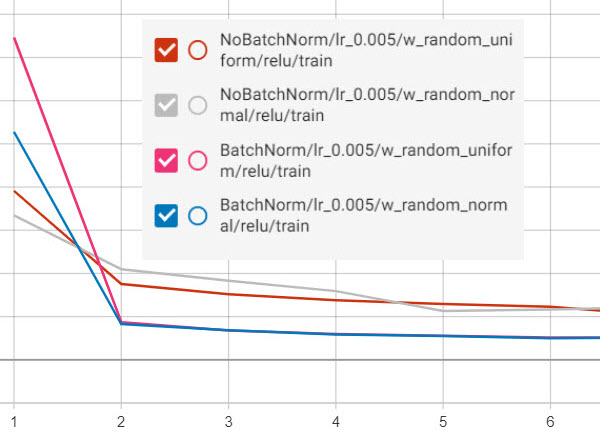
\includegraphics[scale=0.31]{pics/batchNorm/BatchNorm_relu_5.jpg}
  \\
  (1) Learning Rate=1e-3, Relu & (2) Learning Rate=5e-3, Relu\\[6pt]
  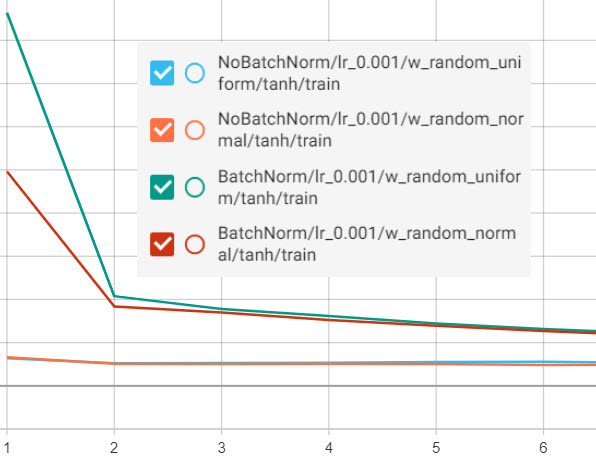
\includegraphics[scale=0.3]{pics/batchNorm/BatchNorm_tanh_1.jpg} &
  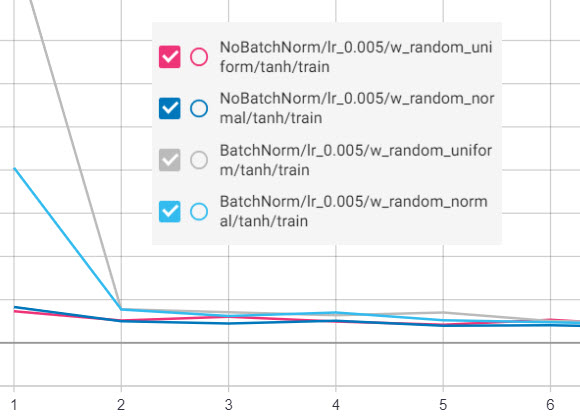
\includegraphics[scale=0.31]{pics/batchNorm/BatchNorm_tanh_5.jpg}\\
  (3) Learning Rate=1e-3, Tanh & (4) Learning Rate=5e-3, Tanh\\[6pt]
\end{tabular}
\caption{Maximum gradient norm among batches w.r.t. one node in the middle layer. Legend in each graph shows whether BatchNorm is applied in the network, what learning rate is used, as well as which activation function. The same random seed for weight initialization is used across all runs.}
\label{fig:maxgradient}
\end{figure}


\section{Discussion}
\subsection{Gradient Confusion}
Gradient confusion is a great quantity to start off with when trying study what methods result in faster, more effective training. Both overparameterized and batch-normalized networks had low gradient confusion, and we were able to justify this through papers outlining rich theoretical reasonings in both cases. The paper by Sankararaman (and other papers related to gradient confusion and other related quantities such as ``gradient diversity'' as introduced by Yin et al \cite{yin}) does not (yet), however, provide any relationships or bounds between gradient confusion and multilayer nonlinear networks; more work should be done in this front, as well as experimentation.

\subsection{Overparameterization}
As shown, overparameterized networks with large widths ($m$) can be regarded as kernel functions. In this paper, we gave strong emphasis on the convergence of gradient descent to global minima in training, both theoretically and experimentally. However, there are still some other aspects which we could have dug into further. For example, Du's\cite{SimonDu} paper argues that the convergence approach can be used for deeper neural networks as well. Arora's \cite{Arora} paper also seems to suggest this. However, Soudry and Carmon's \cite{SoudryCarmon} work seems to show that for multi-layer neural networks, there is no global convergence. Currently, there is not much proof as to whether convergence to global minima would work for multi-layer networks. Another aspect that is relatively obvious (but profound) in this discussion is that in our study of overparameterization, width $m$ has been required to be magnitudes larger than the training set size $n$. In reality, for training neural networks on large training sets (where, nowadays, several datasets range in size on the order of millions), it would be interesting to see what kind of guarantees can be made with smaller $m$. Moreover, our discussion on convergence has been primarily within the training stage, not the testing stage. As to serve the needs of minimizing the population risk, generation bounds would be a good concept to consider for overparameterization as well. 


\subsection{BatchNorm}
Santurkar et al.'s paper \cite{landscape} both empirically and theoretically shows that the optimization landscape of a layer with BatchNorm is smoother than that without BatchNorm. BatchNorm was proven to improve Lipschitzness of loss gradients in deep neural networks. However, in this paper, the proof is based on the somewhat restrictive assumption that $\partial\hat{\mathcal{L}}/\partial z_j = \partial\mathcal{L}/\partial y_j$. Although both $z_j$ and $y_j$ are pre-activations, further justification is needed to make such an assumption. Moreover, even if the assumption is valid for a network with one BatchNorm layer, it's highly likely that in a full BatchNorm network (where BatchNorm is added to all hidden layers) $\partial\hat{\mathcal{L}}/\partial z_j$ differs from $\partial\mathcal{L}/\partial y_j$.

We also question the restrictiveness of the four assumptions made in Kohler et al.'s paper \cite{decoupling}. The first assumption is feasible when the input data is subtracted from its mean. Assumption 2 evidently does not always hold; however, in their experiment using non-Gaussian data, they still are able to show that the results are valid. Assumption 3 is valid for tanh and sigmoid activations; in contrast, RELU is not differentiable at 0. However, the probability that a point is exactly zero is provably zero. Therefore, Assumption 3 is also feasible for the three enumerated popular activation functions we have mentioned. Last, the validity of Assumption 4 is due to further proof. 

In addition, we extended the loss landscape experiment to a full BatchNorm network. By checking the shape of the gradient norm change over each epoch at one node with different learning rates, our results imply that when training BatchNorm network, one should be confident to take larger learning rate. Large learning rates ensure smoother loss changes over epochs, as well as sounder test accuracies.

Another observation is that the training time of BatchNorm network is two to three times as much as that of the regular network. Since experiments in other papers have observed that BatchNorm reduces the number of needed training epochs by a factor larger than three, when training a high-capacity network, the overall training speed is expected to be accelerated by BatchNorm.

\section{Conclusion}
In this paper, we gave a complete survey of theoretical and empirical analyses of overparameterization, batch normalization, and their effects on gradient confusion, which has a direct correlation on training speed. We first introduced the idea of \textbf{gradient confusion}, as well as existent theoretical background that shows precisely why overparameterizing a network by increasing width leads to lowering gradient confusion and thus speeding up training. We gave a new, concise expression that captures the relationship between width and gradient confusion by directly applying Chebyshev's inequality. Next, we transitioned into the theory of \textbf{overparameterization}, and explored convergence guarantees to global minima in training of overparameterized networks. We showed how gradient descent can converge more quickly within the overparameterization context, and we also precisely defined what distinguishes local and global minima in this case. We discussed existing experiments, and we also discussed how we conducted our own experiments in order to verify results of other papers. Lastly we discussed \textbf{batch normalization}. We started with a discussion of how batch normalization empirically affects gradient confusion, thus speeding up training. Next, we defined how the BatchNorm mechanism works in inference. Then, we tackled batch normalization from a theoretical perspective at multiple angles. We discussed how the loss landscape is smoother for networks that have BathNorm layers. We went into detail about how BatchNorm is equivalent to rewriting weights of a network in such a way that decouples length and direction. We highlighted the limitations of BatchNorm, and how these limitations have been addressed in recent research (WeightNorm, LayerNorm, and GroupNorm). Finally, we included our own experiments with many more learning rate and activation function combinations in order to not only verify the theoretical results, but also to show how the gradient norms smoothened in BatchNorm networks, and how gradient norms overall became smaller, specifically in the case of larger learning rates.

\newpage

\medskip

\small

\begin{thebibliography}{9}
\bibitem{Arora}
S.Arora, Simon S.Du, W.Hu ,Z.Li.,R.Wang(2019).\textit{Fine-Grained Analysis of Optimization and Generalization for Overparameterized Two-Layer Neural Networks}

\bibitem{layernorm}
J.L. Ba, J.R Kiros \& G.E Hinton (2016) Layer Normalization. \textit{arXiv:1607.06450}

\bibitem{bassily}
Bassily, R., Belkin, M., \& Ma, S. (2018). \textit{On exponential convergence of SGD in non-convex over-parametrized learning}. arXiv preprint arXiv:1811.02564.

\bibitem{chen}
Chen, L., Wang, H., Zhao, J., Papailiopoulos, D., \& Koutris, P. (2018). \textit{The effect of network width on the performance of large-batch }. In Advances in Neural Information Processing Systems (pp. 9302-9309).

\bibitem{SimonDu}
Simon S.Du,X.Zhai.,B. Poczos.,A.Singh.(2019).\textit{Gradient Descent Provably Optimizes Over-parameterized Neural Networks}

\bibitem{batchnorm} 
S. Ioffe \& C. Szegedy (2015) Batch Normalization: Accelerating Deep Network Training by Reducing Internal Covariate Shift \textit{ICML}

\bibitem{decoupling} 
J. Kohler, H. Daneshmand, A. Lucchi et. al. (2019) Exponential convergence rates for Batch Normalization:The power of length-direction decoupling in non-convex optimization. 	\textit{Proceedings of Machine Learning Research, PMLR 89:806-815.}

\bibitem{Milman}
Milman, V. D., \& Schechtman, G. (2009). \textit{Asymptotic theory of finite dimensional normed spaces: Isoperimetric inequalities in Riemannian manifolds} (Vol. 1200). Springer.

\bibitem{oymak}
Oymak, S., \& Soltanolkotabi, M. (2018). Overparameterized Nonlinear Learning: Gradient Descent Takes the Shortest Path?. arXiv preprint arXiv:1812.10004.
 
\bibitem{reparameter}
T. Salimans \& D.P. Kingma. (2016) Weight normalization: A simple reparameterization to accelerate
training of deep neural networks. \textit{In Advances in Neural Information Processing Systems (NIPS)}.

\bibitem{gradient_confusion}
Sankararaman, K. A., De, S., Xu, Z., Huang, W. R., \& Goldstein, T. (2019). \textit{The Impact of Neural Network Overparameterization on Gradient Confusion and Stochastic Gradient Descent}. arXiv preprint arXiv:1904.06963.

\bibitem{landscape} 
S. Santurkar, D. Tsipras, A.Ilyas \& A. Madry (2018) How Does Batch Normalization Help Optimization? \textit{32nd Conference on In NeurIPS}

\bibitem{SoudryCarmon}
D.Soudry, Y.Carmon(2016).\textit{No bad local minima:Data independent training error guarantees for multilayer neural networks}

\bibitem{Weinan2}
Weinan.E, Chao M.,Lei W.(2019).\textit{A Comparative Analysis of the Optimization and Generalization Property of Two-layer Neural Network and Random Feature Models Under Gradient Descent Dynamics}

\bibitem{Weinan1}
Weinan.E, Chao M.,Lei W.(2019).\textit{A Priori Estimates For Two-layer Neural Networks}

\bibitem{groupnorm}
Y. Wu \& K. He (2018) Group Normalization \textit{European Conference on Computer Vision (ECCV)}

\bibitem{fmnist}
Xiao, H., Rasul, K., \& Vollgraf, R. (2017). Fashion-mnist: a novel image dataset for benchmarking machine learning algorithms. arXiv preprint arXiv:1708.07747.

\bibitem{yin}
Yin, D., Pananjady, A., Lam, M., Papailiopoulos, D., Ramchandran, K., \& Bartlett, P. (2017). \textit{Gradient diversity: a key ingredient for scalable distributed learning}. arXiv preprint arXiv:1706.05699.


\end{thebibliography}






\end{document}

